%!TEX root = mb.tex


\section{Introduction}\label{sec:intro}


    Network processing appliances (``middleboxes'') such as firewalls, proxies, and intrusion detection systems are crucial components of modern networks~\cite{aplomb}. 
     In recent trends, more and more organizations have been {\it outsourcing} their network processing, either to cloud providers~\cite{aplomb, aryaka, zscalar} or to service providers through Network Functions Virtualization (NFV)~\cite{nfv} who now run  middleboxes for the organizations. This strategy promises to reduce costs, decrease the burden of managing and configuring these devices, and provide elasticity and fault tolerance, as documented in~\cite{aplomb}.
Already now, the NFV working group~\cite{nfvwg} has over 250 members ranging from large telecoms to hardware manufacturers, all of whom are investing in new technologies to enable outsourced traffic processing.
   
   Nevertheless, outsourcing middleboxes to the cloud brings a new and important challenge: the confidentiality of the traffic. In order to be able to process and examine the traffic of an organization, the cloud  receives  the traffic {\em unencrypted}.  This means that the cloud now has access to potentially sensitive packet payloads,  IP addresses, and ports revealing confidential information about the organization. This situation is worrisome considering the amount of documented data breaches by cloud employees or hackers gaining access to clouds~\cite{XXX}.
   Hence, an important question is: is it possible to enable a third party to perform traffic processing for an enterprise, {\em without seeing the enterprise's traffic}?
   
   
   

% Justine's text unchanged: (the above is a combination of Justine & Raluca)
%    Network processing appliances (''middleboxes'') such as firewalls, proxies, and intrusion detection systems make up a substantial fraction of modern network infrastructure; studies show that as much as 1/3 of enterprise network hardware consists of such devices~\cite{aplomb}.
%    However, recent trends suggest that this fraction may begin to decline as more and more networks begin to {\it outsource} their network processing, either to cloud providers~\cite{aplomb, aryaka, zscalar} or to service providers through Network Functions Virtualization (NFV)~\cite{nfv}.
%    At the time of this writing, the NFV working group~\cite{nfvwg} has over 250 members ranging from large telecoms to hardware manufacturers, all of whom are investing in new technologies to enable outsourced traffic processing.
%    For consumers, outsourcing traffic processing offers many of the same benefits that outsourcing compute and storage have attained through cloud computing: decreased costs, ease of management, the ability to scale and failover on demand, \etc{}.
%    Nevertheless, outsourcing network processing brings new challenges, and among them, an issue which is critical to most enterprises: privacy.
%    
%    Under traditional middlebox deployments, traffic is processed and inspected by devices which are owned, hosted, and managed entirely within the enterprise itself.
%    Encrypted traffic is often decrypted to enable deep packet inspection (DPI) such as intrusion detection and exfiltration detection.
%    This configuration places critical trust in the hands of network administrators, who can potentially read or even modify {\it any} connection within the company.
%    Outsourcing shifts this trust away from network administrators who are employed and monitored by the company whose data is being processed, and to a third party company with its own employees, hiring practices, and motivations.
%    Hence, in this paper, we ask: is it possible to enable a third party to perform traffic processing for an enterprise, without transferring the ability to read and monitor the enterprise's traffic?
%    
% 
     
     \qu{service provider or cloud? change in title, text and figures}
     
     
  
    We design and build \sys (read ``embark"), the first system that enables running a wide range of middleboxes at a cloud provider while maintaining the confidentiality of the traffic against an attacker with access to all cloud data.  \sys's name concatenates the words MB (middlebox) and Ark (protection). \sys supports a wide range of middleboxes, in fact, all middleboxes that~\cite{aplomb} documents to be fit for cloud outsourcing. These are: firewall, NAT, intrusion detection systems (IDS), data exfiltration systems, web proxy, load balancing, IP forwarding and VPN. \sys supports these applications with competitive performance. 
    
    The approach in \sys is to encrypt the traffic that goes to  the middleboxes in the cloud and enables the cloud to process encrypted traffic without ever decrypting it. \sys encrypts the packet payload as well as important information in the header (such as IP addresses, ports). Since the cloud receives only encrypted traffic and no decryption key, it cannot see the confidential data. However, designing a practical system that supports a wide-range of middlebox applications over encrypted traffic is challenging and required a set of new techniques.
    
    
    
    
\begin{table}[t!]
\centering
\begin{tabular}{p{3.2cm}|p{2.9cm}|p{1cm}}
{\bf Application}  & {\bf Operations used} & {\bf Details} \\
\hline \hline
IP Firewall &   range  & \S\ref{sec:firewall} \\
Application Firewall & range, keyword  & \S\ref{sec:firewall}\\
NAT & range  & \S\ref{sec:nat} \\
IP Forwarding  & range & \S\ref{sec:other_apps} \\
Load Balancer L4 & range & \S\ref{sec:loadb}\\
Load Balancer L7  & range & \S\ref{sec:loadb}\\
Web Proxy/Cache  & keyword & \S\ref{sec:proxy}\\
Intrusion Detect (IDS)  & range, keyword & \S\ref{sec:IDS}\\
Data Exfiltration  & keyword & \S\ref{sec:IDS} \\
VPN Gateway &  none & \S\ref{sec:vpn} \\ 
\end{tabular}
\caption{Middlebox applications supported by \sys and the type of match it needs to perform. Each application is further described in the section specified. \label{tab:apps-ops} }
\end{table}


\begin{figure*}[t!]
\centering
\subfigure[Enterprise to external site communication]{
  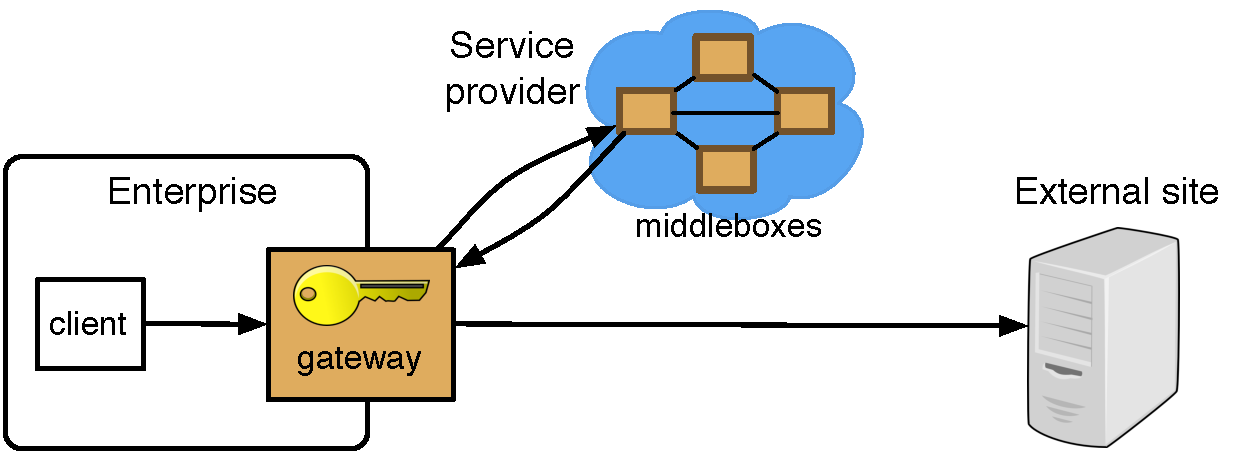
\includegraphics[width=3.3in]{fig/model_1.pdf}
  \label{fig:model1} }
%
\hfill  
\subfigure[Enterprise to enterprise communication]{
   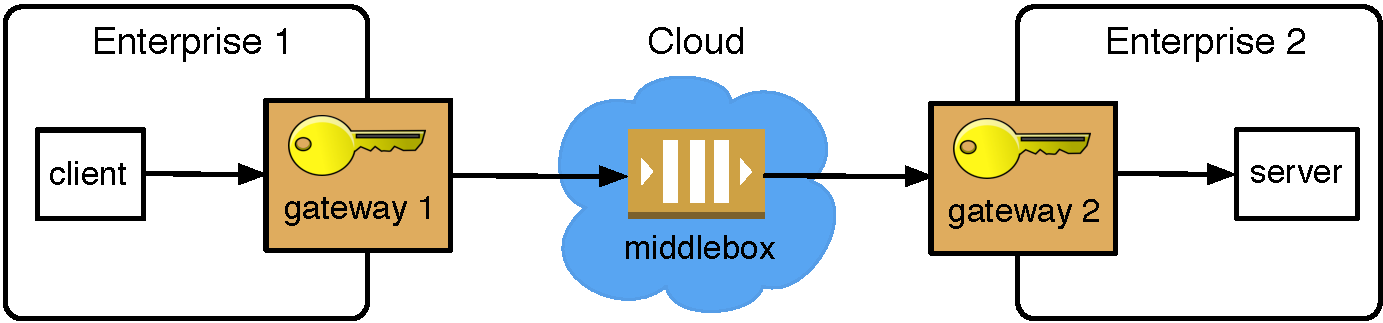
\includegraphics[width=3.1in]{fig/model_2.pdf}
     \label{fig:model2}}
     
     %
\caption{System architecture. Aplomb and NFV system setup with \sys encryption  at the gateway. The arrows indicate traffic from the client to the server; the response traffic follows the reverse direction. \label{fig:sys-overview}}
\end{figure*}

    \subsection{Challenges, techniques, and contributions}
    
    \todo{be careful talking about IDS here too much -- make the BlindBox distinction clear}
The first challenge is that performing generic computation on encrypted data is prohibitively practical. The applications considered provide complex functionalities. For example, firewall and NAT examine packet header information such as IP addresses and ports; for IDS and data exfiltration detection, the middlebox (MB) examines the packet payload and tries to match complex rules (keyword matching, offset information,  regular expressions, etc). The existing generic homomorphic encryption schemes are many orders of magnitude impractical~\cite{aesFHE}.

Fortunately, recently, a recent paper, CryptDB~\cite{popa:cryptdb}, put forth a new vision for building practical such systems, and we are inspired by this vision too. Instead of using a generic encryption scheme, the idea is to identify core operations that underlie the functionality of the system and to support each with a specialized and fast encryption scheme. Unfortunately, neither the core operations nor the encryption schemes in CryptDB fit in our network setting so we need to start from zero.

We study the relevant middlebox applications, and we managed to identify two core operations that underlie all these middleboxes: {\em keyword match} and {\em range match}. Keyword match (KW match) refers to  identifying if a keyword appears in a byte stream at some offset. There are two types of keyword match: regular and cross-boundary. Since we are dealing with network packets, a keyword may appear across two different packets (e.g., ``alice'' appears at the boundary of the packets ``I see ali'' and ``ce at the zoo''.). For example, keyword match is useful for data exfiltration when a watermark is searched for in the traffic, for IDS when malicious strings are searched for in the traffic and for web proxy for matching file identifiers that could be potentially in a cache. 
Range match enables determining if a value $x$ is in an interval ($x_1$ and $x_2$). An example middlebox that uses range match is the firewall.   For example, the firewall has to determine if a source IP address from a packet falls in a certain range of IP addresses and apply a certain action to the packet.  Note that range match supports a basic version of KW match, complete equality check, when the range consists of only one value.
%
Table~\ref{tab:apps-ops} summarizes the middleboxes we support and the operations they rely on. 

A second challenge is that, unfortunately, there is no suitable encryption scheme for these two schemes: either this primitive does not exist, or it is too slow or too insecure for our setting. Performing a regular keyword match can be implemented using searchable encryption~\cite{song, blindbox, X}, which has been studied extensively in the security literature.
However, there is no practical encryption scheme that enables the cross-boundary match. 
For this, we designed a new encryption scheme that is practical and provides the same security guarantee as the regular match -- as if the match is not happening across packet boundaries. 

Regarding range match, the closest encryption scheme is order preserving encryption (OPE)~\cite{mope, BCLO}. However, OPE schemes are too slow for our setting and also leak the order of the values encrypted. We designed a new scheme, called {\em RangeMatch} which is fast (XXX faster than state of the art OPE schemes) and more secure because it does not reveal the order of values encrypted. Interestingly, this scheme is actually a systems technique more than an encryption scheme: it leverages no cryptography, but crucially  exploits the specific systems setup using a carefully-chosen encoding and data structure.

The last challenge is to design and build a system that supports the variety of applications mentioned, is practical and easy to deploy. 
To address this challenge, we make the following contributions:
\begin{itemize}
\item we provide a  protocol for each of the applications in Table~\ref{tab:apps-ops} by employing our two match  primitives,
\item we design each of these protocols and we integrate these protocols in a way that {\em does not change the existing packet structure}. We achieve this by ensuring that our encrypted values fit into the space of the unencrypted values, add layers of headers to packets, and sometimes add a second network flow.
\item  we keep {\em unchanged  the middleboxes that require specialized hardware}, such as the firewall, and enable them to run unchanged on encrypted traffic. Modifying this hardware burdens deployment and could affect performance. 
\end{itemize}


\subsection{Implementation and evaluation}

We implemented and evaluted \sys. As mentioned, we support all applications fit in the cloud outsourcing model, as surveyed in~\cite{aplomb}. PERFORMANCE HERE
